% EN48 c02 | 原书 p.13 中部–p.23 上部（PDF 22–32） | 第 1 章 §1.3
% 块骨架：标题行已设定，正文由译者填写。每页起首用 % ===== 原书 p.N ===== 注释标记。
% 边界说明：按 Lead 批复的方案 A，本块收 §1.3 的全部 30 条结果（自本条首的定义至末条注），
% 止于原书 p.23 上部的末条注；§1.4 自 p.23 中部起，归 c03。
\subsection{环簇的背景}

% ===== 原书 p.13 =====
SYZ 镜像 $Y$ 的构造用到环簇这一套工具：先得到簇 $\tilde Y$，再令
$Y := \tilde Y/\Gamma_B$。环簇提供一种组合式的办法，用来产生定义流形所需的
坐标卡与过渡函数。

下文要在 $Y$ 上定义辛形式。这是给 $Y$ 配备深谷范畴、再用该范畴证明 HMS 的第一步。
% ===== 原书 p.14 =====
由于 $Y$ 局部上是环簇 $\tilde Y$ 按离散群取商的结果，而由多面体构造出的环簇天然
带有线丛，我们就用该线丛的截面定义一个度量。这个度量将给出辛形式。

我们先建立定义该线丛所需的理论。下面是行动路线。
\begin{center}
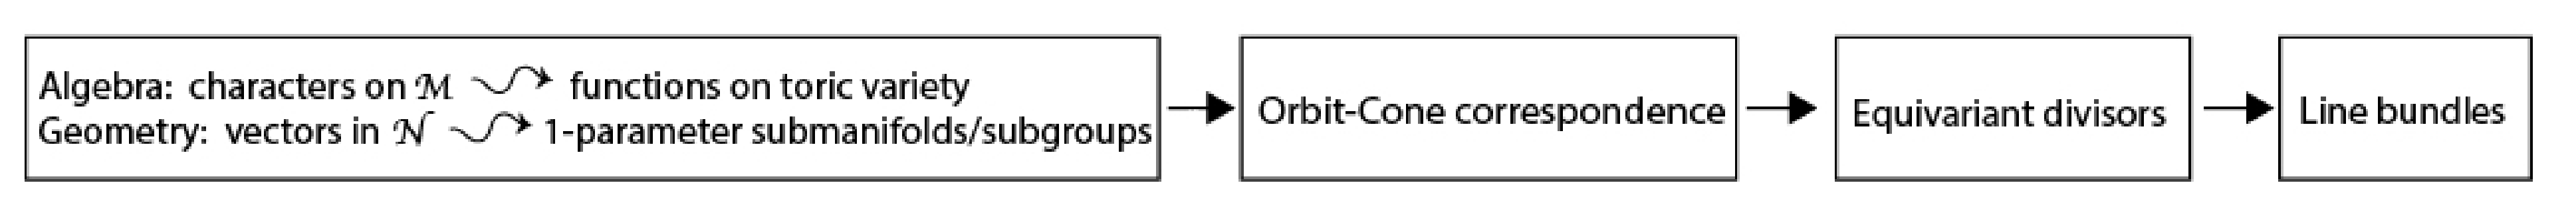
\includegraphics[width=0.98\textwidth]{figures/fig_c02_plan.png}
\end{center}
本小节的背景取自 [CLS11, p 59, p128] 与 [Ful93, Chapter 1]。

\transnote{上图把本节要建立的两条线索并排列出：左栏是代数侧，$M$ 中的特征标给出
环簇上的函数；左栏下一行是几何侧，$N$ 中的向量给出单参数子群。中栏到右栏是推导
路线：先证轨道–锥对应，再由它得到等变除子，最后由除子得到线丛。}

\medskip\noindent\textbf{特征标与单参数子群}\par

设 $Y_\Delta$ 为与多面体 $\Delta$ 相伴的环簇，其构造下文说明。本文对
$Y_\Delta = \PP^2(3)$（即 $\PP^2$ 在三点处爆破）以及后文描述的另一个无限型环簇
[KL19] 使用这套理论。轨道–锥对应解释组合数据（锥）如何给出几何数据（轨道）。
这些数据分别编码在两个向量空间里：特征标空间 $M_\R$，其元素是 $Y_\Delta$ 上的
函数；以及「余特征标」空间 $N_\R$，它生成 $Y_\Delta$ 中的单参数子群（PS）。
下标 $\R$ 表示把格与 $\R$ 作张量积。在这个环簇的代数几何设定里，$M$ 是「代数」，
$N$ 是「几何」。

\begin{definition}[记号]\label{def:notation}
我们固定一些记号。下文将考虑 $n=2$ 与 $n=3$ 的例子。
\begin{itemize}[leftmargin=2.2em,itemsep=0.25em]
\item 几何：$N := \Z^n$，其向量编码环面 $T_N := (\C^*)^n$ 中由 $\C^*$ 参数化的
  单参数子群；该环面在环簇中稠密。有 $N\otimes_\Z\C^* = T_N$ 与
  $N_\R := N\otimes_\Z\R$。
\item 代数：$M = \Hom_\Z(N,\Z)$ 同时编码 $N$ 上的线性泛函（组合层面）与环簇上的
  函数（流形层面）。在 [AAK16] 中，$M$ 的元素称为权向量，因为将其指数化得到
  环簇单项式，而后者是特征标，即环簇上的函数。
\item $M_\R = \R^n$，并由 $\ip{e_i}{f_j} = f_j(e_i) = \delta_{ij}$ 定义非退化配对
  $M_\R\times N_\R\to\R$。
\end{itemize}
\end{definition}

\begin{definition}[锥]\label{def:cone}
锥 $\sigma\subset N_\R$ 是一族半空间
$H_u^+ := \{n\in N_\R\mid \ip{u}{n}\ge 0\}$ 的交，其中 $u$ 取遍 $M$ 中一组法向量。
例如取 $u_1 = e_1$、$u_2 = e_2$，就得到第一象限 $e_1,e_2\ge 0$。于是 $\sigma$ 由
若干格向量的凸线性组合构成；这些格向量称为射线 $\rho$，其全体记作 $\sigma(1)$。

对偶锥 $\sigma^\vee\subset M_\R$ 定义为对偶半空间的交：
\[
\sigma^\vee := \{m\in M_\R\mid \ip{m}{n}\ge 0\ \forall n\in\sigma\}
= \bigcap_{n\in\sigma(1)}\{m\in M_\R\mid \ip{m}{n}\ge 0\}.
\]
\end{definition}

% ===== 原书 p.15 =====
\begin{definition}[强凸有理多面体锥]
强凸指 $\sigma$ 不由任何方向 $e$ 上的 $\pm e$ 生成（等价地，
$\sigma\cap(-\sigma)=\{0\}$）；有理指 $\sigma$ 有整生成元，即生成元都在 $\Z^n$ 中。
\end{definition}

\begin{remark}
若 $m_1,\dots,m_s$ 生成 $\sigma^\vee$，则它们就是 $\sigma$ 中那些半空间的法向量，
即 $\sigma = H_{m_1}^+\cap\cdots\cap H_{m_s}^+$。于是要点在于：$\sigma^\vee$ 把这些
法向量整体编码起来，它的边是 $\sigma$ 的刻面。更一般地，$\sigma$ 中的面 $\tau$
对应 $\sigma^\vee$ 中一个维数互补的面，记作 $\tau^*$，即
$\tau^\perp\cap\sigma^\vee$；反之亦然。
\end{remark}

\transnote{这里「它的边是 $\sigma$ 的刻面」是对偶关系，不是说两者是同一族子集：
$\sigma$ 的刻面（余维 $1$ 的面）与 $\sigma^\vee$ 的边（1 维面）一一对应，且
$\dim\tau + \dim\tau^* = n$。读后文关于多面体刻面的定义时，可以回头对照这一条。}

\begin{definition}[特征标]\label{def:character}
令 $S_\sigma := \sigma^\vee\cap M$ 为对偶锥中的格点。坐标环 $\C[S_\sigma]$ 的元素是
局部定义在 $Y_\Delta$ 上的函数，称为特征标或环簇单项式。它们是集合
$\{\chi^u\mid u\in S_\sigma\}$ 中元素的 $\C$-线性组合。在环簇上定义开集
\[
U_\sigma := \operatorname{Spec}\C[S_\sigma].
\]
特别地，由于 $S_\sigma$ 是半群（可以相加，且含零元），元素 $\chi^u$ 的集合具有
自然的环结构，符合我们对函数坐标环的预期。
\end{definition}

\begin{remark}[记号]
我们用字母 $u$ 表示 $N$ 中的格点。字母 $m$ 保留给 $M_\R$ 或 $M$ 中的点，$n$ 表示
$N_\R$ 中的元素。这样做与 [CLS11] 一致。
\end{remark}

\begin{definition}[仿射卡与函数]\label{def:affine-chart}
$Y_\Delta$ 上的仿射卡（或局部卡）是 $\operatorname{Spec}\C[S_\sigma]$。特别地，
所有局部卡都包含稠密环面
$(\C^*)^n = \operatorname{Spec}\C[\chi^{\pm e_1},\dots,\chi^{\pm e_n}]$，因为
\[
M = \operatorname{Span}_{\Z_+}\langle \pm e_1,\dots,\pm e_n\rangle
\supset \{u\in\sigma^\vee(1)\},
\]
并且射线生成半群 $S_\sigma$。局部函数由特征标 $\chi^u$ 给出。特征标是从稠密环面
到 $\C^*$ 的同态：
\[
\chi^u\colon(\C^*)^n\to\C^*,\qquad
(t_1,\dots,t_n)\mapsto t^u := t_1^{u_1}\cdots t_n^{u_n},\qquad
u = \sum_{i=1}^n u_i e_i.
\]
固定 $S_\sigma$ 的一组基 $\{u_1,\dots,u_k\}$，意思是
$\{\pm u_1,\dots,\pm u_l,u_{l+1},\dots,u_k\}$ 在 $\Z_+$ 上生成 $S_\sigma$，且
$\{u_1,\dots,u_k\}$ 之间没有关系（即极小生成元）。若 $\sigma$ 是强凸锥，就得到带
局部复坐标 $\chi^{u_1},\dots,\chi^{u_k}$ 的坐标卡：
\[
(\chi^{u_1},\dots,\chi^{u_k})\colon U_\sigma\to\C^k.
\]
\end{definition}

\transnote{第一行的包含关系里，$\operatorname{Span}_{\Z_+}\langle
\pm e_1,\dots,\pm e_n\rangle$ 其实就是整个 $M$（因为允许 $\pm e_i$，$\Z_+$ 系数
等于 $\Z$ 系数）。所以任何一张仿射卡都含稠密环面，卡与卡之间的差别只在额外加了
哪些 $\chi^u$。集合 $\sigma^\vee(1)$ 指对偶锥的射线（1 维面）的生成元。}

\begin{remark}
这个卡的像可能是 $\C^k$ 中一个可能奇异的 $n$ 维子簇。特别地，对极大锥有 $k=n$，
$u_i$ 构成 $M$ 的一组 $\Z$-基，于是得到一个光滑簇，以及通常意义上的仿射流形卡，
它把 $U_\sigma$ 映到
% ===== 原书 p.16 =====
局部模型 $\C^n$。

另一种情形是 $u_i$ 不构成 $M$ 的 $\Z$-基，此时它们之间有关系。具体地，
\[
\C[S_\sigma]\cong \C[\chi^{u_1},\dots,\chi^{u_k}]/I,
\]
其中 $I$ 是记录这些关系的环簇理想。下文的 $\PP^2$ 例子（例~\ref{ex:cp2-fan}）
不需要对环簇理想取商。

适当取这个卡的闭包即得环簇。后文会考察特征标何时延拓为整个环簇上的函数，
即 $(\C^*)^n$ 的部分或完全紧化：我们让坐标趋于 $0$ 或无穷。这说明了 $M$ 如何
产生函数。
\end{remark}

\begin{definition}[环簇]\label{def:toric-variety}
回忆锥 $\sigma$ 给出仿射卡。扇是一族锥，其排列方式告诉我们如何粘合局部卡，
即流形上的过渡函数是什么。扇是 $N_\R$ 中的一族锥 $\sigma_i$，满足
\begin{itemize}[leftmargin=2.2em,itemsep=0.25em]
\item 每个锥的每个面都是锥；
\item $\tau_{ij} := \sigma_i\cap\sigma_j$ 是 $\sigma_i$ 与 $\sigma_j$ 共同的面，
  因此沿 $U_{\tau_{ij}}$ 把 $U_{\sigma_i}$ 与 $U_{\sigma_j}$ 粘合。
\end{itemize}
设 $\sigma_1,\sigma_2$ 是两个极大锥，使 $\tau = \sigma_1\cap\sigma_2$ 为 $(n-1)$ 维。
\end{definition}

\begin{claim}\label{claim:tau-hyperplane}
$\tau = H_m\cap\sigma_1 = H_m\cap\sigma_2$，其中
$m\in\sigma_1^\vee\cap(-\sigma_2)^\vee\cap M$。
\end{claim}

特别地，半群 $S_\tau$ 现在含 $\pm m$ 两个方向，而 $\sigma_1$ 只含 $m$、$\sigma_2$
只含 $-m$。这相当于在第一张卡 $\C[S_{\sigma_1}]$ 中把坐标 $\chi^m$ 取逆、在第二张卡
$\C[S_{\sigma_2}]$ 中把坐标 $\chi^{-m}$ 取逆；两者现在都要求非零。我们沿
\[
U_\tau = (U_{\sigma_1})_{\chi^m} = (U_{\sigma_2})_{\chi^{-m}}
\]
粘合这两张卡。

\transnote{两张卡各自的坐标是 $\chi^m$ 与 $\chi^{-m}$，它们互为倒数；要求非零就是
要求取出这两张卡的交。后文例~\ref{ex:cp2-fan} 的过渡映射 $g_{12}$ 正是把这个取逆写成坐标
变换，即 $\chi^{(1,0)}\mapsto 1/\chi^{(1,0)}$。}

由此可以看出 $N$ 如何产生单参数子群。

\begin{definition}[单参数子群（1-PS）]\label{def:one-parameter}
给定 $v = \sum_{i=1}^n v_i f_i\in N$，通过乘法同态得到单参数子群 $\lambda^v$：
\[
\lambda^v\colon \C^*\to(\C^*)^n,\qquad t\mapsto(t^{v_1},\dots,t^{v_n}).
\]
例如 $v=(1,1)$ 给出复单参数子群 $(t,t)_{t\in\C^*}\subset(\C^*)^2$。取
$(\chi^{u_1},\dots,\chi^{u_k})$ 在 $\{\lambda^v(t)\}_{t\in\C^*}$ 上的像，
就得到 $U_\sigma$ 中的一维子流形。
\end{definition}

\begin{remark}
把特征标与单参数子群复合，得到 $\C^*$ 的特征标：
\[
\chi^u\circ\lambda^v(t) = t^\ell,\qquad \ell = \ip{u}{v}.
\]
特别地，把所有单参数子群收集起来，即可几何地看出 $N$ 就是稠密环面：
\[
N\otimes_\Z\C^*\colon v\otimes t\mapsto\lambda^v(t).
\]
\end{remark}

% ===== 原书 p.17 =====
\begin{example}[$\PP^2$]\label{ex:cp2-fan}
扇有三个锥，其射线分别由 $v_1 = f_1$、$v_2 = f_2$、$v_3 = -f_1-f_2$ 在 $N_\R$
中生成。
\begin{center}
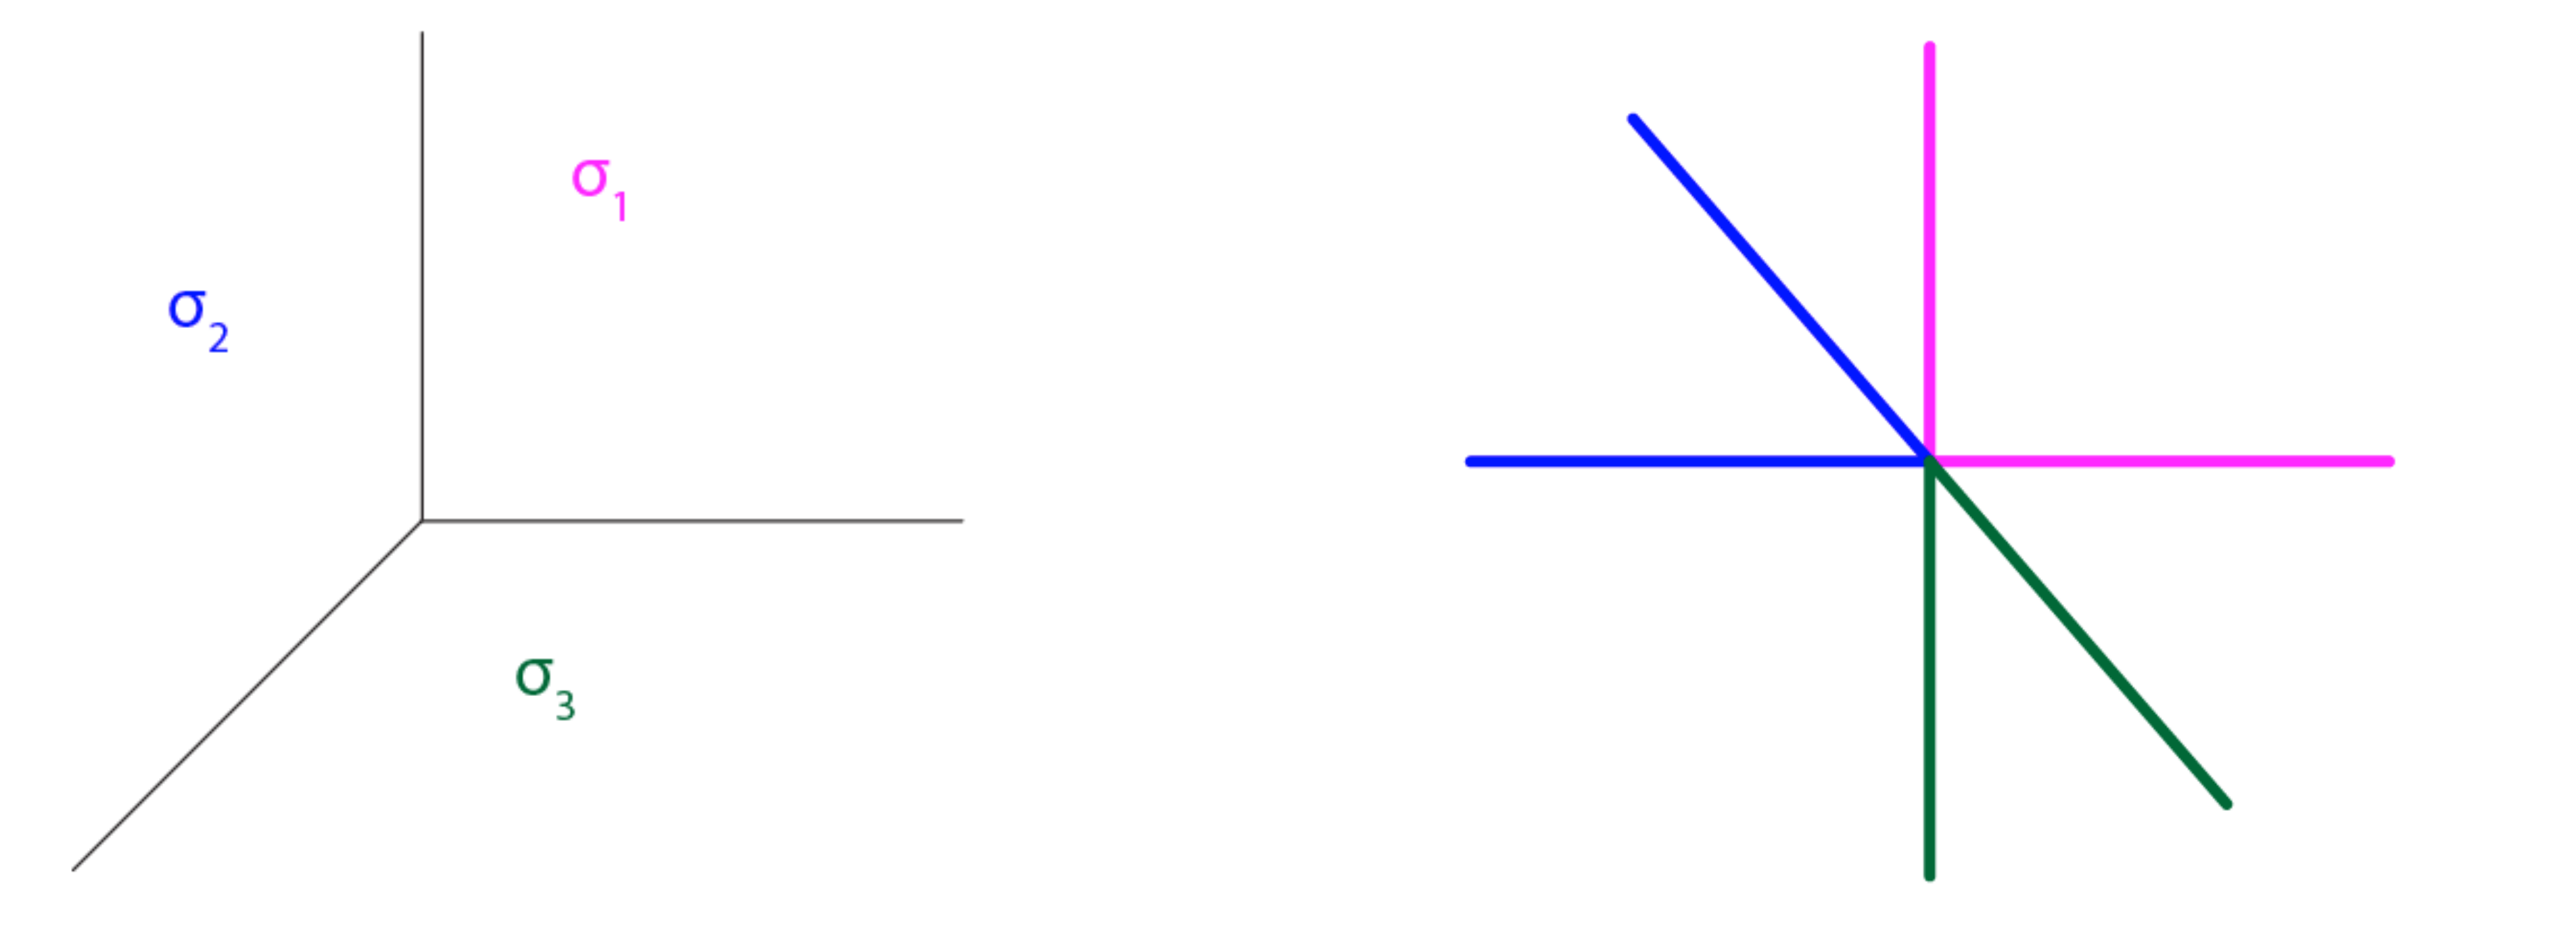
\includegraphics[width=0.86\textwidth]{figures/fig_c02_fan.png}
\end{center}
在原锥上取非负值的线性泛函，其对偶锥为
\begin{gather*}
\sigma_1^\vee = \operatorname{span}(e_1,e_2),\\
\sigma_2^\vee = \operatorname{span}(-e_1,-e_1+e_2),\\
\sigma_3^\vee = \operatorname{span}(-e_2,e_1-e_2).
\end{gather*}
这些对中的向量之间没有关系，所以它们对应某个同构于 $\C[x,y]$ 的仿射卡的变量。
换言之，我们不需要对记录生成元之间关系的环簇理想 $I$ 取商。每种情况下选取生成元，
就给出卡上的一个复坐标。
\begin{align*}
U_{\sigma_1} &= \operatorname{Spec}\C[\chi^{1,0},\chi^{0,1}]\cong\C^2
\ni(\chi^{1,0},\chi^{0,1}),\\
U_{\sigma_2} &= \operatorname{Spec}\C[\chi^{-1,0},\chi^{-1,1}]\cong\C^2
\ni(\chi^{-1,0},\chi^{-1,1}),\\
U_{\sigma_3} &= \operatorname{Spec}\C[\chi^{0,-1},\chi^{1,-1}]\cong\C^2
\ni(\chi^{0,-1},\chi^{1,-1}).
\end{align*}
若 $\tau = \sigma_1\cap\sigma_2$，则这相当于把 $\chi^{1,0}$ 取逆，并且
$\tau^\vee = H^+_{(1,0)}$。选定生成元就选定了坐标；两种不同的自然选择给出坐标变换：
\begin{align*}
\C[S_{\sigma_1}] &= \C[\chi^{(1,0)},\chi^{(0,1)}]
\subset \C[\chi^{\pm(1,0)},\chi^{(0,1)}] = \C[S_\tau]\\
&\rightsquigarrow \operatorname{Spec}\C[\chi^{\pm(1,0)},\chi^{(0,1)}]
\to \operatorname{Spec}\C[\chi^{(1,0)},\chi^{(0,1)}],
\end{align*}
以及
\begin{align*}
\C[\chi^{-(1,0)},\chi^{(-1,1)}] &\subset
\C[\chi^{\pm(1,0)},\chi^{(-1,1)}]\\
&\rightsquigarrow \operatorname{Spec}\C[\chi^{\pm(1,0)},\chi^{(-1,1)}]
\to \operatorname{Spec}\C[\chi^{-(1,0)},\chi^{(-1,1)}].
\end{align*}
注意 $\C[\chi^{\pm(1,0)},\chi^{(0,1)}] = \C[\chi^{\pm(1,0)},\chi^{(-1,1)}]$，
在 $\operatorname{Spec}$ 下得到 $U_\tau$。选定生成元给出与 $\C^*\times\C$ 的一个
等同；两张卡中的这个等同再作为恒等映射嵌入 $\C^2$。这个等同的两种不同选择给出
过渡映射：
\[
g_{12}(\chi^{(1,0)},\chi^{(0,1)}) :=
\left(\frac{1}{\chi^{(1,0)}},\ \frac{\chi^{(0,1)}}{\chi^{(1,0)}}\right).
\]
这样就回到我们对 $\PP^2\ni[z_0:z_1:z_2]$ 的理解，其中
$\chi^{(1,0)} = z_1/z_0$，$\chi^{(0,1)} = z_2/z_0$。
\end{example}

\transnote{两串包含与 $\operatorname{Spec}$ 的图说的是同一件事：$U_{\sigma_1}$ 与
$U_{\sigma_2}$ 各自嵌入 $U_\tau$，而 $U_\tau$ 等同 $\C^*\times\C$。把第二串的坐标
换回第一串的坐标就得到 $g_{12}$，这正是 $\PP^2$ 的标准过渡函数：$\C^*\times\C$
里一点在第一张卡上记作 $(\chi^{(1,0)},\chi^{(0,1)})$，在第二张卡上记作其倒数。}

% ===== 原书 p.18 =====
\medskip\noindent\textbf{轨道–锥对应}\par

要理解等变除子，需要理解组合数据如何给出几何数据。除子对应簇上某个坐标的零点。
这一点可以从扇通过「轨道–锥对应」读出。

\begin{lemma}[轨道–锥对应]\label{lem:orbit-cone}
环簇中某点的 $n-k$ 维 $(\C^*)^n$-轨道，与扇的 $k$ 维锥之间存在一一对应；
例如除子与射线对应。
\end{lemma}

\begin{proof}
思路是：「对应于 $N$ 中某个锥内部的点的每个单参数子群，都收敛到同一个极限点。」
（回忆定义~\ref{def:one-parameter} 中 $N$ 的点与单参数子群的对应。）该点给出确定
单参数子群方向的向量。按代数几何，环簇上的一个点是半群同态
$S_\sigma = \C[\sigma^\vee\cap M]\to\C$，即映射
$\operatorname{Spec}\C\to U_\sigma$。回忆 $M$ 编码环簇上的函数。因此，这样的赋值
确定了所有函数在该点的取值；知道一个点处所有函数的取值，与知道这个点本身是同样的
信息。给定 $v\in\sigma\cap N$，用 $\sigma^\vee\cap M$ 的一组基上的如下映射，可以给
相应的点指定坐标：
\[
\sigma^\vee\cap M\ni u\mapsto\lim_{t\to0}\chi^u(\lambda^v(t))
= t^{\ip{u}{v}}\in\C.
\]
下面用一条断言说明：一个锥的所有向量为何给出同一个极限点。由此，取该锥的极限点
的轨道，就得到轨道–锥对应。

\begin{claim}\label{claim:limit-point}
由方向 $v\in\operatorname{int}(\sigma)\cap N$ 给出的所有单参数子群都收敛到同一点。
\end{claim}

\begin{proof}
为清楚起见，我们用下标 $u_{\mathrm{bdry}}$、$u_{\mathrm{int}}$ 区分需要对每个 $v$
核对的两种函数（即 $u$ 不在对偶锥 $\sigma^\vee\subset M$ 的内部，或 $u$ 在其内部）。
可以看到：
\begin{enumerate}[leftmargin=2.6em,itemsep=0.3em]
\item $u_{\mathrm{bdry}}\in\sigma^\vee\cap\sigma^\perp$ 推出对一切 $v\in\sigma$ 有
  $\ip{u_{\mathrm{bdry}}}{v}=0$，因此
  \[
  \lim_{t\to0}\chi^u(\lambda^v(t)) = t^{\ip{u}{v}} = 1.
  \]
\item $u_{\mathrm{int}}\in\sigma^\vee\setminus(\sigma^\vee\cap\sigma^\perp)$ 推出：
  一方面，按 $\sigma^\vee$ 的定义，对一切 $v\in\operatorname{int}(\sigma)\cap N$
  有 $\ip{u_{\mathrm{int}}}{v}\ge 0$；另一方面，对 $\sigma$ 内部的 $v$ 有
  $\ip{u_{\mathrm{int}}}{v}\ne 0$，且 $u_{\mathrm{int}}\notin\sigma^\perp$。因此
  \[
  \lim_{t\to0}\chi^u(\lambda^v(t)) = t^{\ip{u}{v}} = 0.
  \]
\end{enumerate}
\end{proof}

为完成轨道–锥对应的证明，令对应锥 $\sigma$ 的轨道为 $(\C^*)^n\cdot p$，其中 $p$
是点
\[
\lim_{t\to0}\bigl(\chi^{u_1}(\lambda^v(t)),\dots,
\chi^{u_k}(\lambda^v(t))\bigr),
\]
$v\in\sigma$，$u_1,\dots,u_k$ 是 $S_\sigma$ 的生成元。由上一条断言，可以任取 $v$。
\end{proof}

\transnote{两个极限的差别全在指数 $\ip{u}{v}$ 上：边界方向使指数为 $0$，极限是
$1$；内部方向使指数严格为正，极限是 $0$。所以「极限点」的各坐标只取 $0$ 或 $1$，
由 $u$ 属于哪一类函数决定。这也解释了为何同一锥的所有方向给出同一点。}

% ===== 原书 p.19 =====
\begin{example}[$\PP^2$]\label{ex:cp2-cones}
扇的锥与对偶锥如下：
\begin{gather*}
\{0\},\quad \{0\}^\vee = M_\R\cong\R^2,\\
\rho_1 = \langle(1,0)\rangle,\quad \rho_2 = \langle(0,1)\rangle,\quad
\rho_3 = \langle(-1,-1)\rangle,\\
\rho_1^\vee = \langle\pm(0,1),(1,0)\rangle,\quad
\rho_2^\vee = \langle\pm(1,0),(0,1)\rangle,\\
\rho_3^\vee = \langle\pm(-1,1),(-1,0)\rangle,\\
\sigma_1 = \langle(1,0),(0,1)\rangle,\quad
\sigma_2 = \langle(1,0),(-1,-1)\rangle,\quad
\sigma_3 = \langle(0,1),(-1,-1)\rangle,\\
\sigma_1^\vee = \langle(1,0),(0,1)\rangle,\quad
\sigma_2^\vee = \langle(0,1),(1,-1)\rangle,\\
\sigma_3^\vee = \langle(-1,0),(-1,1)\rangle.
\end{gather*}
生成与锥 $\sigma$ 对应的轨道的极限点 $\gamma_\sigma$，是把
$\sigma^\perp\cap\sigma^\vee$ 中的向量 $m$ 送到 $1$、把 $\sigma^\vee$ 中其余向量
送到 $0$ 的点。令 $(t_1,t_2)\in(\C^*)^2$ 为稠密环面轨道上的坐标。对 $S_{\rho_i}$
所取的生成元列在下面的指数中。
\begin{align*}
\lambda^{(0,0)}(t) &= (1,1), &
\gamma_{\{0\}} &= \lim_{t\to0}(\chi^{(1,0)}(1,1),\chi^{(0,1)}(1,1))
= (1,1) \Longrightarrow (\C^*)^2,\\
\lambda^{(1,0)}(t) &= (t,1), &
\gamma_{\rho_1} &= \lim_{t\to0}(\chi^{(0,1)}(t,1),\chi^{(1,0)}(t,1))
= (1,0) \Longrightarrow \C^*\times\{0\},\\
\lambda^{(0,1)}(t) &= (1,t), &
\gamma_{\rho_2} &= \lim_{t\to0}(\chi^{(1,0)}(1,t),\chi^{(0,1)}(1,t))
= (1,0) \Longrightarrow \C^*\times\{0\},\\
\lambda^{(-1,-1)}(t) &= (t^{-1},t^{-1}), &
\gamma_{\rho_3} &= \lim_{t\to0}(\chi^{(-1,1)}(t^{-1},t^{-1}),
\chi^{(-1,0)}(t^{-1},t^{-1})) = (1,0) \Longrightarrow \C^*\times\{0\}.
\end{align*}
在环簇中取闭包，就得到三个环簇除子，即 $(\C^*)^n$ 作用不变的除子。
\end{example}

\transnote{表中每行左边是单参数子群 $\lambda^v$，右边是它给出的极限点。第三、四行的
第一分量都趋于 $1$，第二分量都趋于 $0$，所以轨道是 $\C^*\times\{0\}$ 型的一维轨道。
$\gamma_{\{0\}}$ 对应零锥，它的轨道就是整个稠密环面 $(\C^*)^2$。}

\begin{claim}\label{claim:orbit-closure}
设 $O(\sigma)$ 表示轨道–锥对应下与锥 $\sigma$ 对应的轨道。则轨道的闭包给出的
环簇除子有如下描述：
\[
\overline{O(\tau)} = \bigcup_{\tau\le\sigma} O(\sigma).
\]
\end{claim}

记号：$N(\sigma)$ 指 $N$ 中的格点模去 $N_\sigma$ 中的格点，其中
$N_\sigma := \sigma\cap N$。

\medskip\noindent\textbf{除子、线丛与多面体}\par

除子–射线对应是轨道–锥对应的特例；按复几何 [Huy05, §2.3]，除子的定义函数给出
线丛的过渡函数。下面引入多面体的概念，并说明它为何决定一个线丛。我们将看到，
它的构造使它的边与扇中的射线垂直，而它的大小控制每个不可约环簇除子（对应扇的
射线）上的系数。这个除子随后给出与该多面体对应的线丛。

\begin{definition}[多面体]\label{def:polytope}
多面体 $P\subset M_\R$ 是
\[
P := \{m\in M_\R\mid \ip{m}{\nu_i}\ge -a_i\}\subset M_\R,
\]
其中 $i$ 取有限多个值，$\nu_i\in N$ 生成扇 $\Sigma$ 的射线 $\rho_i$。若 $i$ 取
无限多个值，更一般地得到多面体（polyhedron）。
\end{definition}

% ===== 原书 p.20 =====
\begin{definition}[面、刻面]
多面体中余维 $1$ 的面称为刻面：对某个 $i$ 有 $\ip{u}{v_i} = -a_i$，且对 $j\ne i$
有 $\ip{u}{v_j} > -a_j$。余维更高的面则对不止一个 $i$ 满足
$\ip{u}{v_i} = -a_i$。
\end{definition}

% [Tutor Note: 本条原文用 v_i 与 u，与定义~\ref{def:polytope} 的 ν_i、以及记号约定中「m 表示
% 多面体侧的点」不一致。此处照录原书符号，不作改动。]

\begin{definition}[由 $P$ 得到扇]\label{def:fan-from-polytope}
（全维格多面体的顶点对应环簇卡，参见 [CLS11, p 76]。）给定顶点为 $\mathbf v$ 的
多面体 $P$，把每个顶点平移为原点，取它的边张成的锥，即
$C_{\mathbf v} := \operatorname{Cone}(P\cap M-\mathbf v)\subset M_\R$。对应的扇中的
锥定义为
\[
\sigma_{\mathbf v} := C_{\mathbf v}^\vee
= \operatorname{Cone}(\nu_i\mid \text{第 } i \text{ 个面包含 } \mathbf v)
\subset N_\R.
\]
于是卡为
$U_{\sigma_{\mathbf v}}
= \operatorname{Spec}\C[\operatorname{Cone}(P\cap M-\mathbf v)\cap M]$。（更一般地，
对多面体的面 $Q$，$\sigma_Q$ 是由包含 $Q$ 的面的 $\nu_i$ 张成的锥。）所以要点是：
「环簇的局部坐标可以从多面体的顶点出发沿它的边读出。」
\end{definition}

检查所有锥 $\sigma_Q$ 的全体确为一个扇，我们把它定义为 $\Sigma_P$。

\transnote{这里的操作分三步：先把多面体平移使某个顶点落在原点，再由该顶点出发的边
张成一个锥 $C_{\mathbf v}$；取对偶锥就落到 $N$ 一侧，得到扇的锥。对偶的作用正是把
「多面体的边」换成「法向量 $\nu_i$」。所以多面体的顶点对应扇的极大锥，而多面体的
面（法向量）对应扇的射线。}

\begin{remark}
关于对偶化 $\sigma\to\sigma^\vee$ 在多面体层面的类比（多面体 → 极多面体），讨论见
[Ful93, §1.5, p 26]。可以把 $M_\R$ 中的多面体 $P$ 过渡到锥
$\operatorname{Cone}(P\times\{1\})\subset M_\R\times\R$，再对锥取对偶 $\vee$，
得到 $N_\R\times\R$ 中的锥；可以证明这是 $P$ 的极 $P^0$ 上的锥，即形如
$\operatorname{Cone}(P^0\times\{1\})$，其中 $P^0\subset N_\R$ 是对偶多面体。
\end{remark}

\transnote{取 $\operatorname{Cone}(P\times\{1\})$ 相当于给多面体加一个高度坐标，
把有界的多面体变成无界的锥；锥的对偶仍在锥的层面进行，所以「多面体对偶」被化归为
「锥对偶」。这与定义~\ref{def:cone} 的对偶锥是同一套操作，只是所在空间多了一维。}

\begin{definition}[等变除子]
等变除子（或 $T$-除子）是环簇轨道闭包的线性组合。
\end{definition}

\begin{claim}
$T$-除子是刻面对应除子的线性组合。
\end{claim}

\begin{proof}
扇的射线对应等变除子。事实上，给定射线 $\rho$，其正交补 $\rho^\perp$ 余维为 $1$；
这意味着特出点 $\gamma_\rho$ 有 $n-1$ 个 $1$ 与 $1$ 个 $0$（其中 $0$ 来自 $\rho$
生成的那个方向，它把余维 $1$ 的空间 $\rho^\perp$ 送到零）。所以 $(\C^*)^n$-轨道是
$(n-1)$ 维的。取它的闭包就得到除子 $D_\rho$，即
\[
D_\rho = \overline{O(\rho)} = \bigcup_{\rho\le\sigma} O(\sigma).
\]
这样就从某个坐标的零点得到了除子。
\end{proof}

\begin{remark}[记号]
既然现在知道 $\nu_i$ 与 $a_i$ 中的 $i$ 由多面体的刻面 $F$ 标号，就可以用 $F$
来标号它们。
\end{remark}

\begin{definition}[特出除子]
设 $P := \{m\in M_\R\mid \ip{m}{\nu_i}\ge -a_i\}\subset M_\R$ 为整多面体，即
$a_i\in\Z$。由轨道–锥对应，可以对 $\Sigma_P$ 中每条射线 $\nu_F$ 取对应轨道的
闭包，得到环簇除子 $D_F$。
\end{definition}

% ===== 原书 p.21 =====
于是可以由这个扇构造环簇 $Y_P$。最后，把 $Y_P$ 中的特出除子定义为
\[
D := \sum_F a_F D_F.
\]

\begin{remark}
整性条件使我们能定义该除子，并在之后把 $Y_P$ 嵌入射影空间，因为 $D$ 将对应一个
丰富线丛。
\end{remark}

\begin{claim}[{$\OO(D)$ 的截面，[CLS11][Proposition 4.3.3]}]\label{claim:sections}
$\OO(D)$ 的截面由
\[
\Gamma(Y_P,\OO(D)) = \bigoplus_{m\in P\cap M}\C\cdot\chi^m
\]
给出，其中 $P := \{m\in M_\R\mid \ip{m}{\nu_F}\ge -a_F\}\subset M_\R$，
$D = \sum_{F\ \text{刻面}} a_F D_F$。
\end{claim}

\transnote{直和只取 $P\cap M$ 中的格点，而不是整个 $P$。这就用上了整性条件
$a_i\in\Z$：它保证 $P$ 是格多面体，各面由格点方程 $\ip{m}{\nu_F} = -a_F$ 切出，
于是 $P\cap M$ 足够大，能用来标号截面。}

\begin{proof}
按定义
\[
\Gamma(Y_P,\OO(D)) = \{f\in\C(Y_P)^*\mid
\operatorname{div}(f)+D\ge 0\}\cup\{0\},
\]
其中 $\C(Y_P)^*$ 由 $Y_P$ 上的可逆有理函数组成。注意
\[
\operatorname{Supp}(D)\cap T_N = \emptyset,
\]
因为 $T_N$ 是所有坐标都非零的轨道，而 $\operatorname{Supp}(D)$ 由 $D_F$ 组成，
后者包含至少一个坐标为零的轨道。因此 $D|_{T_N} = 0$，且
$\operatorname{div}(f)|_{T_N}\ge 0$，即 $f$ 是 $T_N = \operatorname{Spec}\C[M]$
上的正则函数。由此推出 $f\in\operatorname{Spec}\C[M]$，从而
\[
\Gamma(Y_P,\OO(D))\subset \C[M].
\]
% [Tutor Note: 原文作 f ∈ Spec C[M]，按上下文应为 f ∈ C[M]；此处照录，不擅改。]

写 $f = \sum_{m\in\mathcal A} c_m\chi^m$，其中 $\mathcal A\subset M$，系数
$c_m\in\C$。注意 $\Gamma(Y_P,\OO(D))$ 是 $T_N$-不变子集，作用为
\begin{gather*}
T_N\curvearrowright\Gamma(Y_P,\OO(D))\colon t\cdot f := f\circ t^{-1},\\
T_N\curvearrowright T_N\colon t\cdot p := (t_1p_1,\dots,t_np_n),
\end{gather*}
因为 $D_F$ 是 $T_N$-不变的，且 $f$ 与 $f\circ t^{-1}$ 的零点集相同。特别地，令
\[
B = \operatorname{span}\{\chi^m\mid m\in\mathcal A\}.
\]
由于 $\chi^m\colon T_N\to\C^*$ 是同态，$T_N$ 保持 $\chi^m$ 张成的空间，因为
\[
t\cdot\chi^m(p) = \chi^m(t^{-1}\cdot p) = \chi^m(t^{-1})\chi^m(p)
\quad\therefore\quad t\cdot\chi^m = \chi^m(t^{-1})\chi^m.
\]
于是 $W := B\cap\Gamma(Y_P,\OO(D))$（由于 $f$ 是有限和，它是有限维的）作为两个
$T_N$-不变子空间的交也 $T_N$-不变。下面用一些线性代数的结果。注意 $T_N$-作用由
有限维空间 $W$ 上的线性映射组成，因而给出两两交换的有限维矩阵（$T_N$ 是交换
% ===== 原书 p.22 =====
群），所以这些矩阵可以同时对角化，即可以找到 $W$ 的一组特征向量基。特别地，
按表示论，可以把表示 $T_N\to\GL(W)$ 写成 $1$ 维表示的直和，即特征标 $\chi^m$。
于是要点是：$f\in W$ 既可以表示成 $\C[M]$ 中特征标之和，也可以表示成 $W$ 中
特征标之和；由唯一性，这两个表达式相同。因此对 $m\in\mathcal A$ 有
$\chi^m\in W$，且
$f\in\bigoplus_{\chi^m\in\Gamma(Y_P,\OO(D))}\C\cdot\chi^m$，从而
\[
\Gamma(Y_P,\OO(D)) = \bigoplus_{\chi^m\in\Gamma(Y_P,\OO(D))}\C\cdot\chi^m.
\]

最后一步如下。取一个整体截面 $\chi^m$。条件
$\operatorname{div}(\chi^m)+D\ge 0$ 在系数上等价于
\[
\ip{m}{\nu_F}+a_F\ge 0.
\]
换言之，这等价于 $m\in P$。但 $\chi^m$ 是特征标意味着 $m\in M$，因此这等价于
$m\in P\cap M$；于是得到最终结果
\[
\Gamma(Y_P,\OO(D)) = \bigoplus_{m\in P\cap M}\C\cdot\chi^m.
\]
\end{proof}

\begin{claim}[{无基点，[CLS11][Proposition 6.1.1]}]\label{claim:basepoint-free}
不存在点 $p\in Y_P$ 使对所有 $m_i\in P\cap M$ 都有 $\chi^{m_i}(p)=0$。换言之，
$\OO(D)$ 无基点，因为
$\Gamma(Y_P,\OO(D)) = \bigoplus_{m_i\in P\cap M}\chi^{m_i}$。
\end{claim}

\begin{proof}
回忆面 $Q\subset P$ 给出描述多面体 $\Sigma_P$ 的扇的锥 $\sigma_Q$。我们要证明：
对每个仿射片 $U_{\sigma_Q}$，存在一个在该片上不为零的整体截面。由于
$U_{\sigma_Q}$ 覆盖环簇，这就够了。

把面 $Q = \bigcap_{F\supset Q} F$ 写成刻面的交。于是
\[
Q := \{m\in M_\R\mid \ip{m}{\nu_F} = -a_F,\ \forall F\supset Q\}\subset M_\R.
\]
取格点 $m_Q\in Q$，例如一个顶点。由断言~\ref{claim:sections}，$\chi^{m_Q}$ 是
$\OO(D)$ 的整体截面。又对 $F\supset Q$ 有 $\ip{m_Q}{\nu_F}+a_F=0$，这意味着
$\chi^{m_Q}+D$ 沿 $U_{\sigma_Q}$ 的零点阶数为零：
\[
(\operatorname{div}(\chi^{m_Q})+D)|_{U_{\sigma_Q}}
= \sum_{F\supset Q}(\ip{m_Q}{\nu_F}+a_F)D_F = 0.
\]
换言之，$\chi^{m_Q}(U_{\sigma_Q})\ne 0$。
\end{proof}

\transnote{「无基点」是说：每个点处至少有一个截面不为零，所以这些截面不会共同消失。
下一推论正是利用这一点，用 $\sum_i|\chi^{m_i}|^2$ 作分母定义 $h$；若分母在某点为零，
$h$ 就没有定义。}

% ===== 原书 p.23 =====
\begin{corollary}[{辛形式的定义，[Huy05][Example 4.1.2]}]\label{cor:symplectic-form}
由断言~\ref{claim:sections} 回忆
\[
\Gamma(Y_P,\OO(D)) = \bigoplus_{m_i\in P\cap M}\chi^{m_i}.
\]
由断言~\ref{claim:basepoint-free}，$\OO(D)$ 无基点，所以这些基元素在任何点
$p\in Y_P$ 处不会同时为零。于是可以定义凯勒形式
\[
\omega_P := \frac{i}{2\pi}\partial\bar\partial h,\qquad
h = \frac{1}{\sum_{i=1}^s|\chi^{m_i}|^2},
\]
其中 $|\cdot|$ 指 $\C$ 中的标准模，因为 $\chi^{m_i}$ 是复坐标。
\end{corollary}

\transnote{这里的 $h$ 不是 $\omega_P$ 的凯勒势，而是它的倒数形式：$\omega_P$ 由
$\partial\bar\partial h$ 给出，$h$ 取截面模长平方和之倒数。$|\cdot|$ 用 $\C$ 的
标准模，是因为 $\chi^{m_i}$ 在所取的卡上是复坐标，不是实坐标。}

\begin{remark}
$\OO(D)$ 是丰富线丛，这意味着 $Y_\Delta$ 可以看成射影空间中的簇。它丰富的原因
可在 [CLS11] 中找到，源于多面体的组合性质。多面体的某个倍数 $kP$ 是正规的
（第 2 章），这推出该多面体是丰富的（第 2 章的定义）；后者随后被证明等价于线丛
丰富（第 6 章）。直观上，极丰富多面体有足够多的格点，对应有足够多的截面来定义
嵌入。
\end{remark}
